
\subsection{Graph parallels. }
Although there are many graph based methods that exist within the reduction realm, most of these concentrate on the generation of skeletal methods through the building of a directed tree (subcategory of graphs from source to target) - LIST of refs and sentence of all skeletal methods. Path flux analysis (Sun et al 2010)\\

Instead we may find ourselves applying graph theory to solve other reduction methods. For instance we can trace back influence through connecting edges using dijkstras shortest path algorithm (CH2 ref) - analogous to the connectivity method, or a leave one out approach combined with pagerank to access the effects of removing a node.\\

We can use the graph structure to analyse changes of reactions or relationships between species. This can provide an alternative representation and method to access such data. Additionally we may use graph clustering techniques to locate groups of highly connected, fast reacting/strongly related species. This has applications in both understanding the data, but more importantly chemical lumping. In creating a graph from the mechanism, we not only encode information about the chemical structure, but also the rate of reaction in the graph. In grouping species by high numbers of reactions between them with fast fluxes we can take a QSSA style approach to reduction, and assume that since the rate of reaction between them is much much faster than those outside a cluster, they may be grouped together. This will be explored in PART II [ref link].



\section{Methodology: Part I }
In this chapter we are not interested in reducing a mechanism for a certain case study or environment. Instead we look at tools capable of simplifying the hard coded maths behind the reactions that exist within the atmosphere. Since the key chemical drivers differ from location to location we make use of our ability to run a range of different simulations which provide an overview of the entirety of the input space (intial concentrations). Although this may not replicate and real-word (physical) scenarios, it tests the robustness of the mathematics behind the mechanism and in using this data to predict like properties based on the physical equations which describe the system. We work on the assumption that these have been correctly fitted and tested against experimental data, and that through reducing the mechanism based purely on its mathematical response to different conditions, its ability to predict atmospheric science will be preserved. \\

The model setup shall be defined below. 

\subsection{The Mechanism}
The mechanism we wish to use as a baseline is the Common Representative Intermediates (CRI) Mechanism of version 2.265 ,\cite{criv2}. This is an update to the CRI v2.0, with the purpose of updating the chemistry to better represent that of MCM version 3.3.1 (i.e. the inclusion of explicit Isoprene chemistry). The CRI v2.265 mechanism has been developed much in the same way as its precursor, and is centred around describing the ozone formation from Volatile organic compounds (VOCs) in the troposphere. The main assumption behind the lumping in the generation of this mechanism is that `the potential for ozone formation from a given volatile organic compound (VOC) is related to the number of reactive (i.e., CC and CH) bonds it contains',\cite{cri}. Reductions are made on a compound-by-compound basis and compared to the MCM using a series of 5 day box-model simulations. \\

The CRI v2.265 mechanism contains 422 species and 1261 reactions. This is still almost double of those within the global GEOS-Chem model. With explicit manual reduction being used to reduce the MCM by YY percent, we wish to apply a series of automated reduction techniques and compare them to the baseline mechanism. We chose the 2.265 version of CRI, since it posesses both a potential for further reduction (CRI v2.0 was reduced a further 5 times); there are a sufficient number of items to make it a non-trivial example, but mainly as its relative size is just within our ability to visually inspect the output of each species. 

\subsection{The Box-Model}
The box model used shall be an adapted version of the Dynamically Simple Model of Atmospheric Chemical Complexity (DSMACC) [ref doi, ref DSMACC]. This has had several changes which allow for multiple parallel runs, easy extraction of rates, fluxes and the jacobian matrix as well as a simple ncurses interface for loading and parsing new files. \\

The DSMACC model works by using the Kinetic Pre Processor (KPP) [REF] to generate Fortran code, which can then be used to integrate the provided mechanism. As there were some issues presented with this a pre-pre parser code was used on the mechanism before running KPP, and a post parser on some of the files to provide the desired output. 

\subsection{Model Inputs}
As we do not wish to constrain results to a specific case example, we provide a range of inputs with the aim of covering all possible concentration combinations. As a means of determining all non-lumped species within the CRI mechanism, we only used those which appear in both the MCM and CRI. This also ensures that should it be desired at a later date, any further reduced mechanisms can directly be compared with the results of the full MCM. \\

In terms of sampling there are several types that may be used ,\cite{sampling}. The main or most common is Random, or Monte Carlo, sampling. The problem with this is that its pseudo random nature may often results in regions of high density and some of low, \autoref{fig:mc}. In attempting to sample the entirety of our input space we use a method based on the principles of a Latin square. A latin square is a square containing n items, arranged in such a way that they only appear once in each row and column, much akin to a sudoku puzzle ,\cite{lsq}. A latin hypercube is a generalisation of this allowing for an alternative subspace sampling to the monte carlo method which expands the probabilistic stratified-style sampling of a latin square into n-dimentional space. This presents better covarage of our input space \autoref{fig:lh}  and will be used with the following limits, TAABLE, to gen our sample simulations.

\begin{figure}[H]

\begin{subfigure}{.5\textwidth}
  \centering
  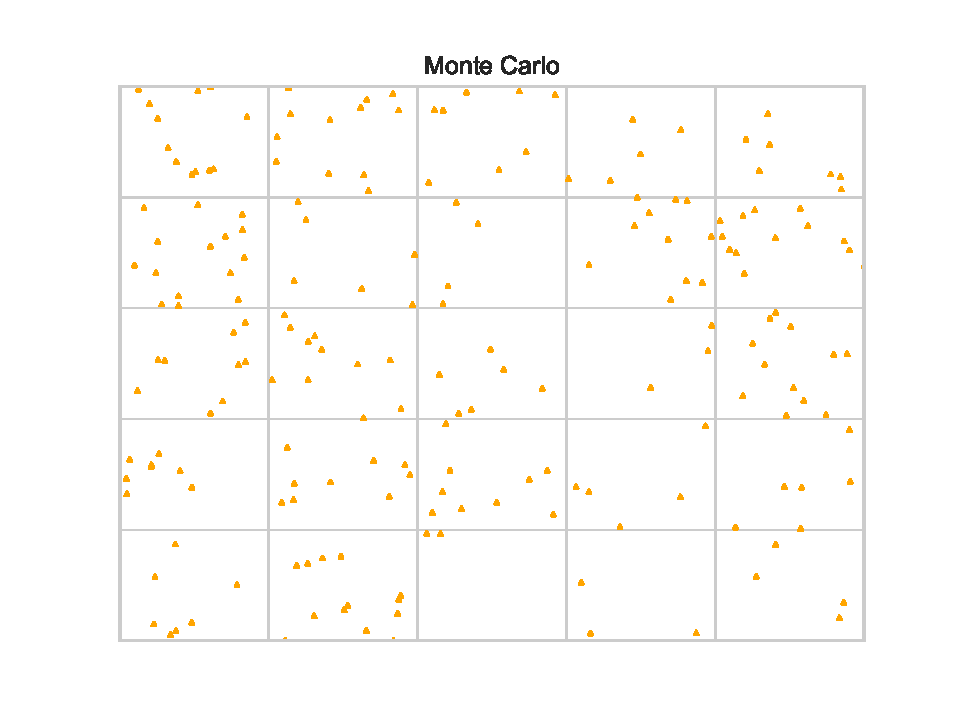
\includegraphics[width=\textwidth]{fig/mc.pdf}
  \label{fig:mc}
\end{subfigure}%
\begin{subfigure}{.5\textwidth}
  \centering
  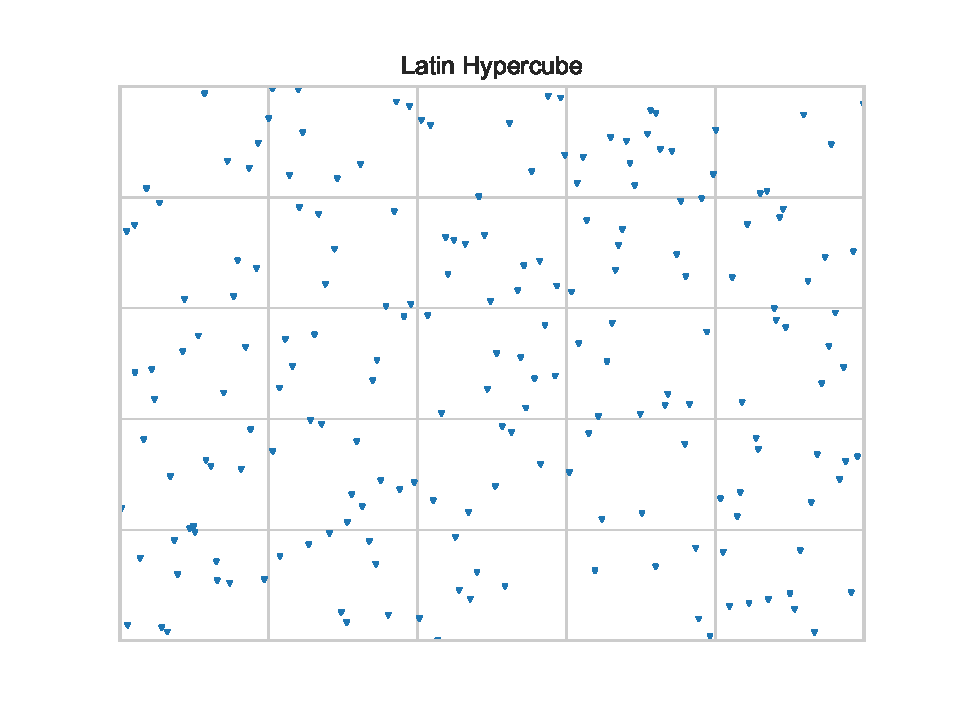
\includegraphics[width=\textwidth]{fig/lh.pdf}
  \label{fig:lh}
\end{subfigure}%

\caption{A comparison of the distribution of 250 sampled points using a) Monte Carlo and b) Latin Hypercube sampling}
\end{figure}


\begin{equation}
\text{concentration}
    \begin{cases}
      min = 10^{-8} \ max=10^{-13} , & \mathbf{if} NO,NO_2,O_3\\
      min = 10^{-8} \ max=10^{-13} , & \text{otherwise}\\
      
    \end{cases}
  \end{equation}

\subsection{Reduction through Lifetime}





\subsubsection{Calculating the lifetime}
Within models a species lifetime is regarded as the time taken for its concentration to halve [ref]. This works on the assumption that the species is not produced, and that rate coefficients and other constants remain constant. For a first order decay of sample \autoref{eqn}, we can represent the decay using \autoref{decay}, showing that the half life is independent of initial concentration. 

\begin{equation}
A \rightarrow{^k} B
\label{eqn}
\end{equation}

\begin{equation}
s(t) = a_0 \exp(-kt) \\
\frac{a(t)}{a_0} = \exp(-kt) \\
$$linearised this gives$$
\ln (\frac{a(t)}{a_0}) = -kt
$$ after $\tau_{1/2}$ the concentration is equal to $a_0/2$ of initial rate $a_0$, which gives $$
\ln(\frac{\frac{a_0}{2}}{a_0}) = \ln(\frac{1}{2}) = \ln(2^{-1}) = -\ln2 = k\tau_{1/2} 
$$$$
\tau_{\frac{1}{2}} = \frac{\ln 2}{k}
\label{decay}
\end{equation}

In species of the first order only, this may simplified to 
\begin{equation}
a(t) = a_0 \exp (t  \sum_j k_j )
$$ and therefore the half life may be written as the reciprocal sum of rate coefficients: $$
\tau_A = 1 / \sum_j k_j
\end{equation}

and is how lifetime is calculated for photochemical species [ref! pillin and seakins]. An alternative method for half life calculation may be obtained using the diagonal (self reference) of a Jacobian matrix ,\cite{kinetics}:

\begin{equation}
\tau_1 = - \frac{1}{J_{ii}}
\end{equation} 

This value will usually be negative unless a species does not contain a consuming reaction, then it will be zero. 


The xxxxx method of reduction consists of the isolation of species with similar lifetimes and reactions as a means of lumping. In doing so the ... etc 


\subsection{Comparing Magnitude and Direction}
Since the photolysis reactions in a model change the resultant rates, and thus flux of a species depending on the azimuthal angle related to the time of day, we not only want to compare species with the same magnitude, they also need to match the profile as they change. To do this we may represent all pariwise species matches on a latent space representing the size and angle between their temporal vectors. This is done through using the euclidean distance on the $x$ axis, and cosine distance $y$ on the $y$. 

\subsubsection{Euclidian distance}
This is the simplest method of vector comparison and works by calculating the distance between all points in two vectors. For the vectors

\begin{equation}
v1 = [ a,b,c, \dots n ] 
$$$$
v2 = [ i,j,k, \dots z ]
\end{equation}

This can be done using pythoagoras' theorem in \autoref{euclid}:

\begin{equation}
e_{dist}  = \sqrt{(a-i)^2 + (b-j)^2 + (c-k)^2 + \dots + (n-z)^2}
\label{euclid}
\end{equation}

This transformation converts the straight line distance between each vector into metric space, allowing us to represent the difference in their magnitudes as a single scalar. Unfortunately as this requires the difference between all permutations of rows, it cannot be done as a single operation, but as multiple. \\

APPLICA"tiion

\subsubsection{Cosine Distance} 

Similarly if we wish to calculate the angle between two vectors we may use the cosine difference. In starting with the definition of the dot product 

\begin{equation}
v1 \cdot v2 = \|v1\|\|v2\| \cos \theta
$$this may be arranged$$
\cos \theta = \frac{ v1 \cdot v2}{\|v1\|\|v2\|}
\end{equation}

Since this does not work for the triangle ? inequality, we need to normalise each vector before calculating the cosine distance. The merits of this come from  ... which makes its application comparing the similarity between texts or documents of different sizes very popular (REF!). \\


COMPARE force graph of cosine differences and force graph of euclidean distances. Colour ones close to eachother. \\



\section{Results: Part I}

In order to get a representation of the mechanism we run 300 randomly initiated scenarios, with the experimental design capable of accepting more data at a later point. We then extract the lifetimes from the diagonal of the jacobian, and convert them into vectors representing the duration of all 3 days for each simulation. These vectors are then compared against eachother to find species of similar lifetimes, which follow a like response to the diurnal cycle. This is done through the use of euclidian and cosine similarities. 

\subsection{Temporal Lifetime Vector Comparison}
First we wish to explore the results of a single simulation. This will help establish the thresholds and methodology that is to be used in future examples. As we do not wish to lump inorganics, we remove these from the program and generate all the pairwise interactions between species. We compute the euclidean and cosine distances for all remaining reaction pairs (88410 pairs) across the entirety of the single calculation. These are then plotted on separate axis, and coloured using the geometric mean, \autoref{fig:metric}. \\

Since there are $n^2$ different combinations, this process can be lengthy to compute. Moreover the number of nodes present makes it difficult to visually determine which couplets to lump together, especially when they are overlaying eachother, as in \autoref{fig:morig}. To overcome this we apply a force graph simulation to each node. Here a strong force pulls them towards their true location, whist a collision/repulsive force ensures that there exists no overlap between nodes. Although some information loss may be incurred this way, it does enable us to interactively determine which pairs belong to which points.   

Plotting the data this way provides an approximate view of how lifetimes change within the system. \autoref{fig:density} shows the distribution of values across both metrics. Here we see that although there is some difference the cosine difference can be used as an indicator for exploring further. This is useful since the cosine difference is a matrix operation and can produce near instant results in the form of the output relationship matrix. The euclidean distance however must be computed for each coupling individually as it requires taking the difference between the temporal lifetime arrays of each species. This means that rather than computing the euclidean distance for all permutaions of species, we can compute only those whose cosine distances suggest potentially promising results.  



\begin{figure}[H]
\begin{subfigure}{.5\textwidth}
  \centering
  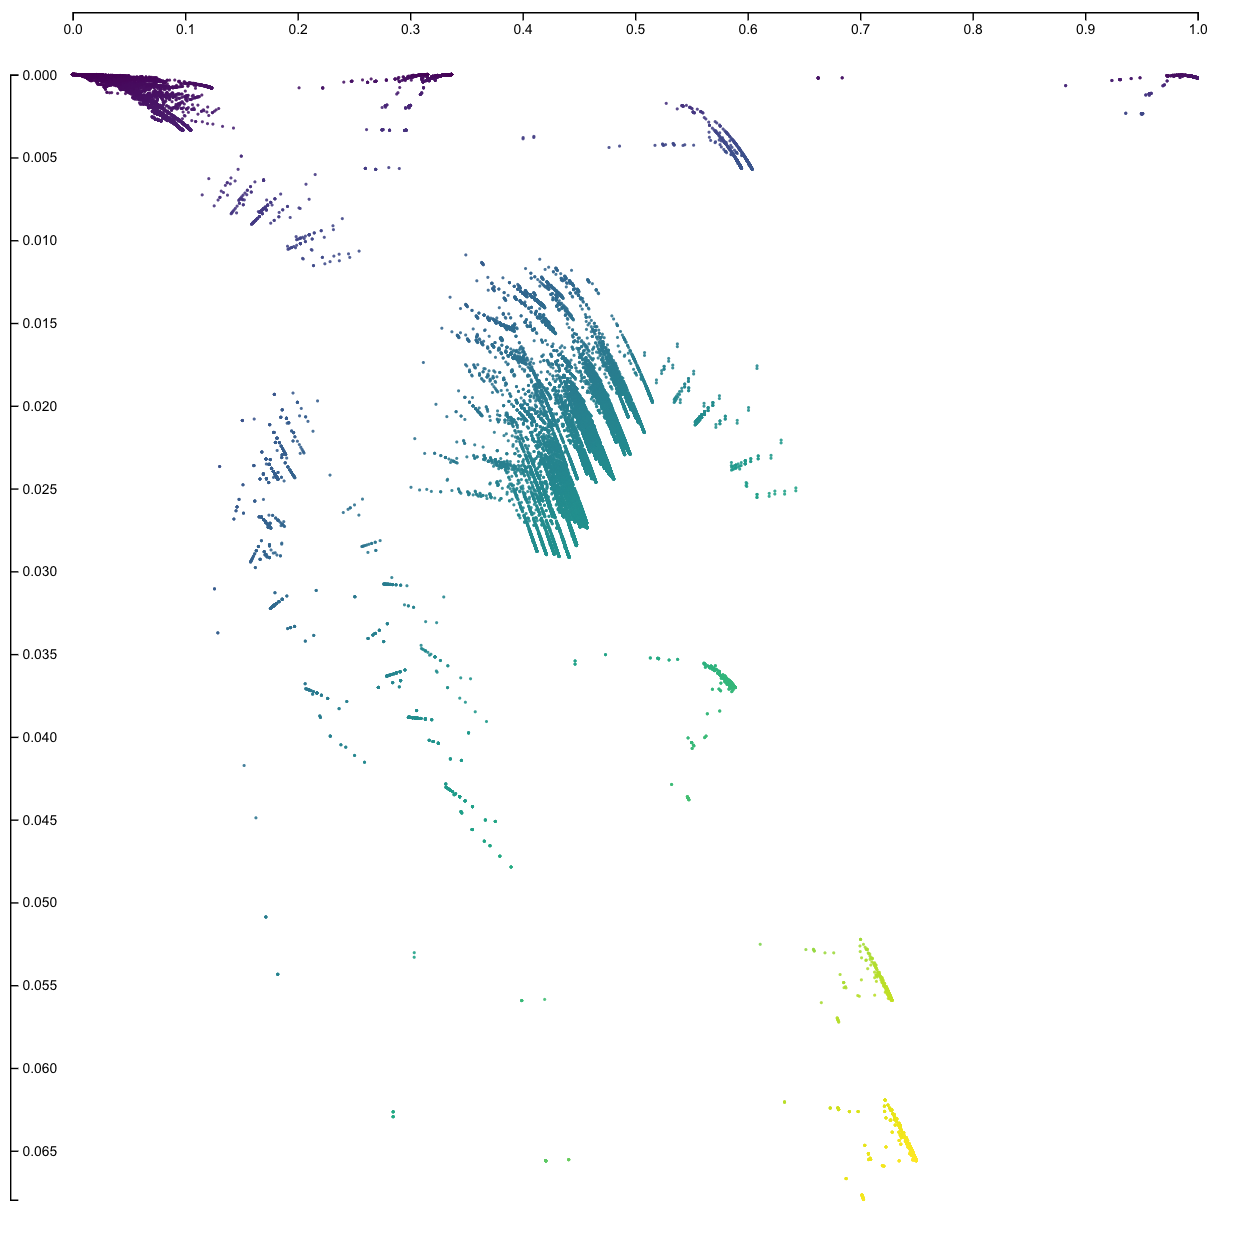
\includegraphics[width=\textwidth]{fig/metric-1.png}
  \label{fig:morig}
  \caption{Original}
\end{subfigure}%
\begin{subfigure}{.5\textwidth}
  \centering
  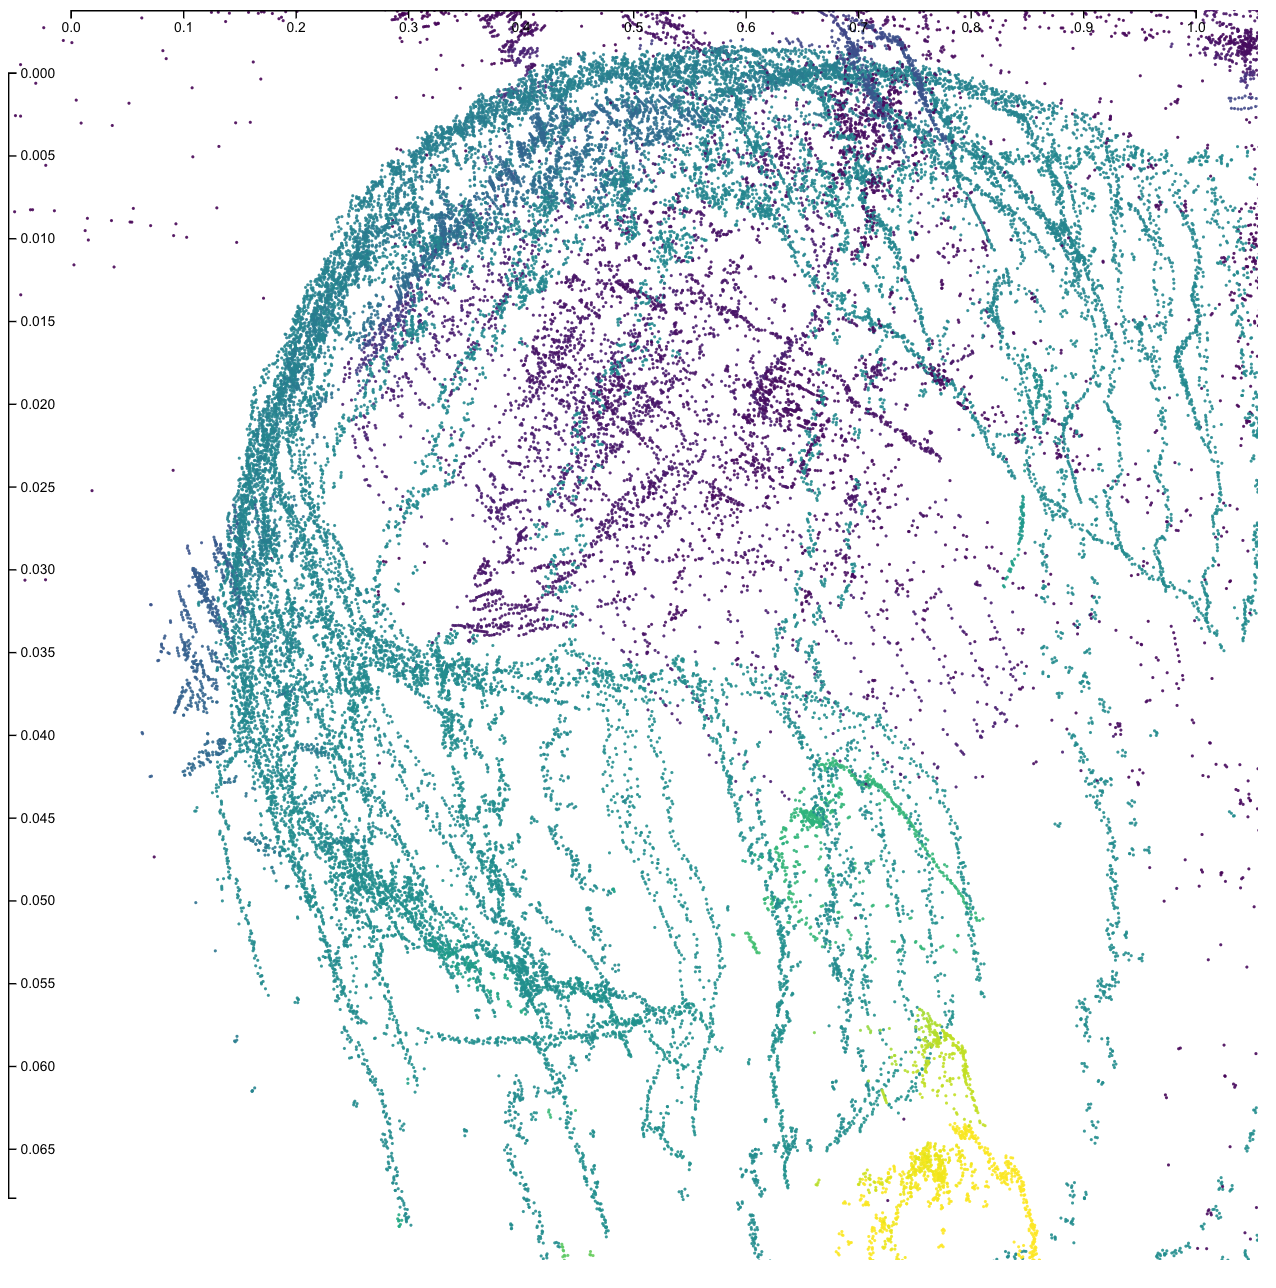
\includegraphics[width=\textwidth]{fig/metric0.png}
  \label{fig:m1}
  \caption{First collision detection timestep, before attractive forces have fully kicked in.}
\end{subfigure}

\caption{Showing the evolution from the original overlaid locations, \autoref{fig:morig} to the slightly more accessible (interactively) \autoref{fig:metric}}
\end{figure}


\begin{figure}

\begin{subfigure}{.5\textwidth}
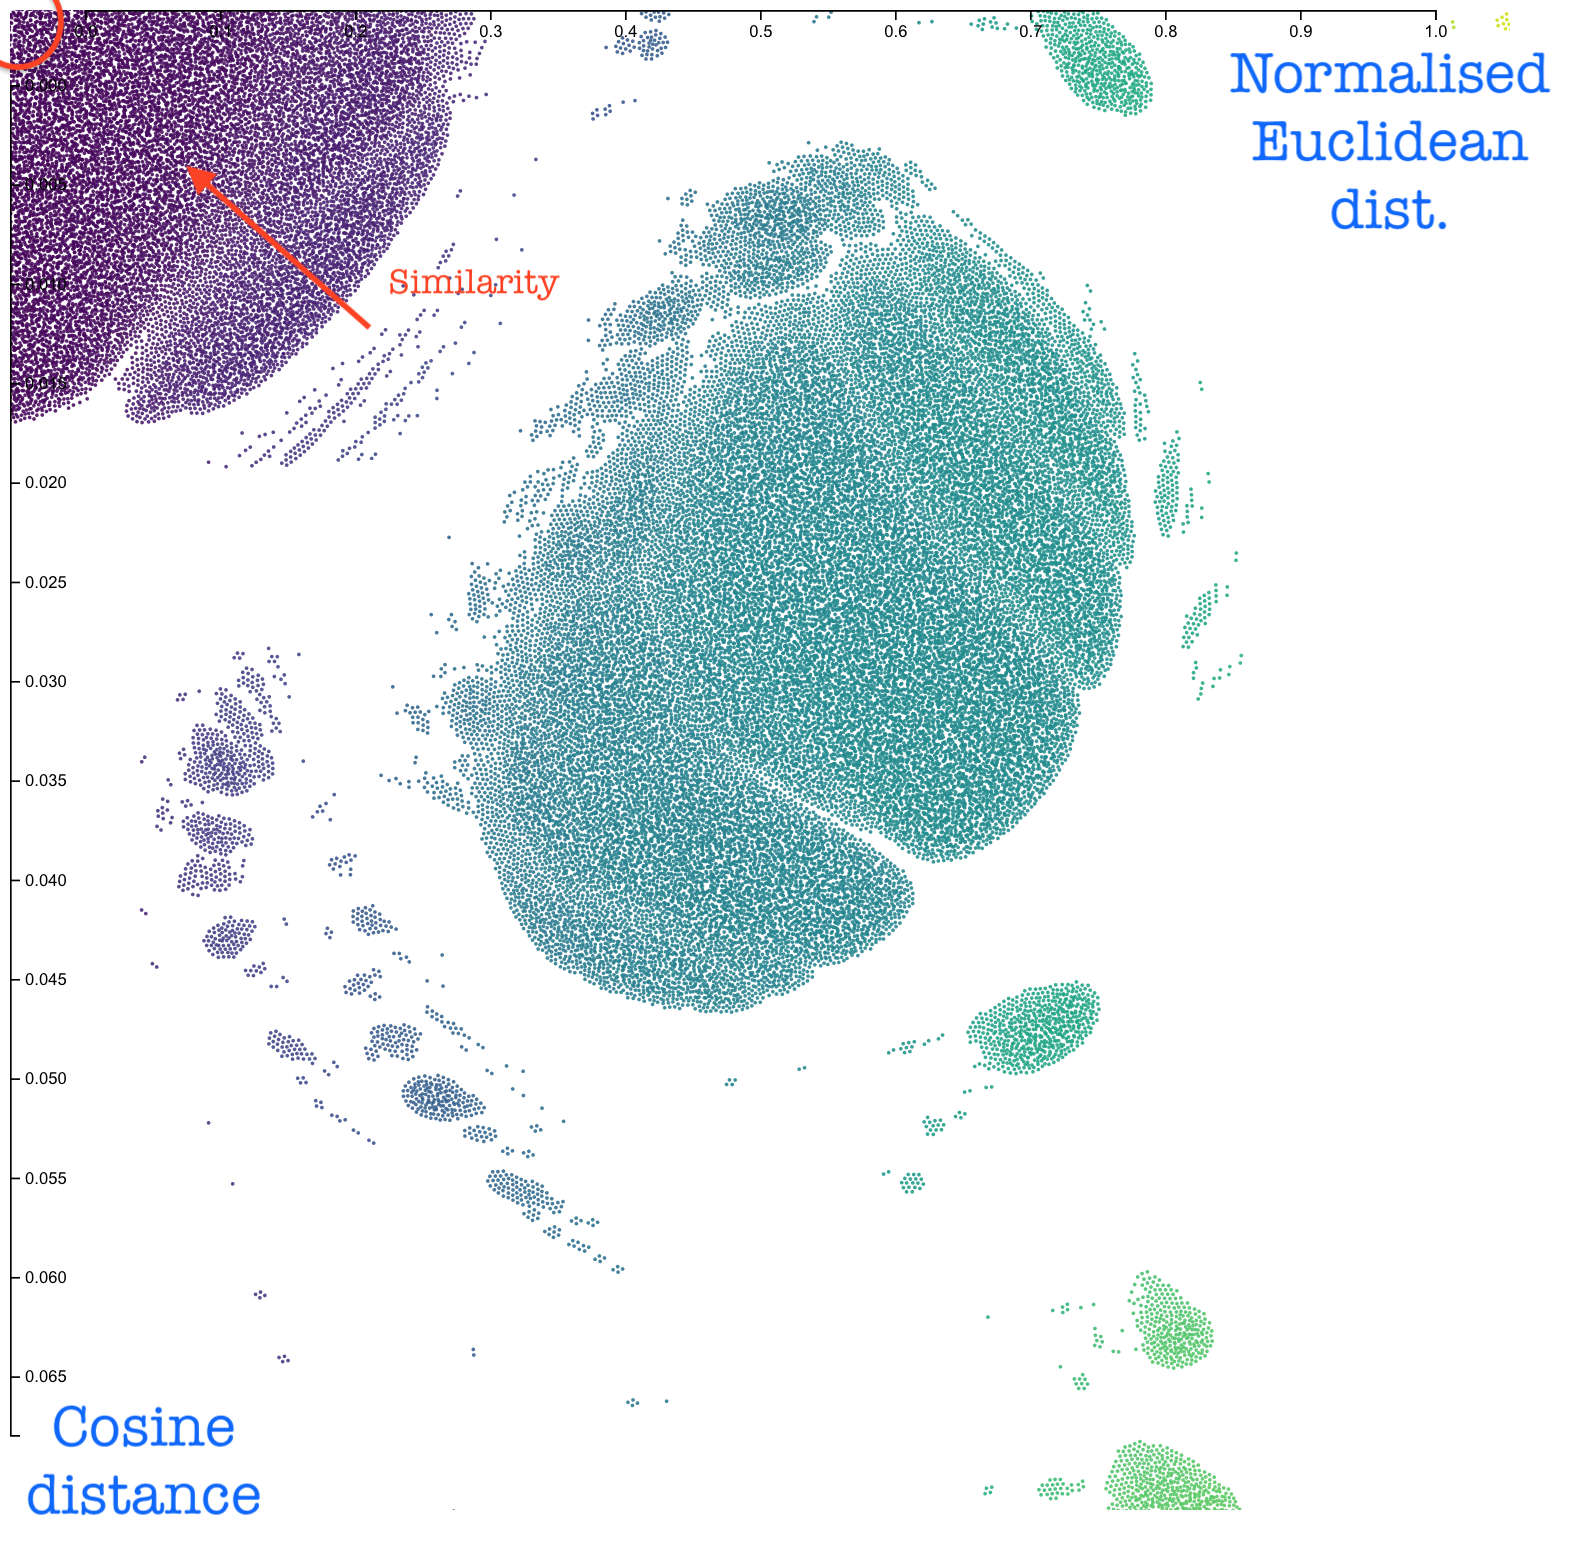
\includegraphics[width=\textwidth]{fig/metric.png}
\label{fig:metric}
\caption{Interactive, non overlapping plot of normalised euclidian distance across the x axis against the cosine distance on the y. The colouring is the geometric mean between them.}
\end{subfigure}
\begin{subfigure}{.5\textwidth}
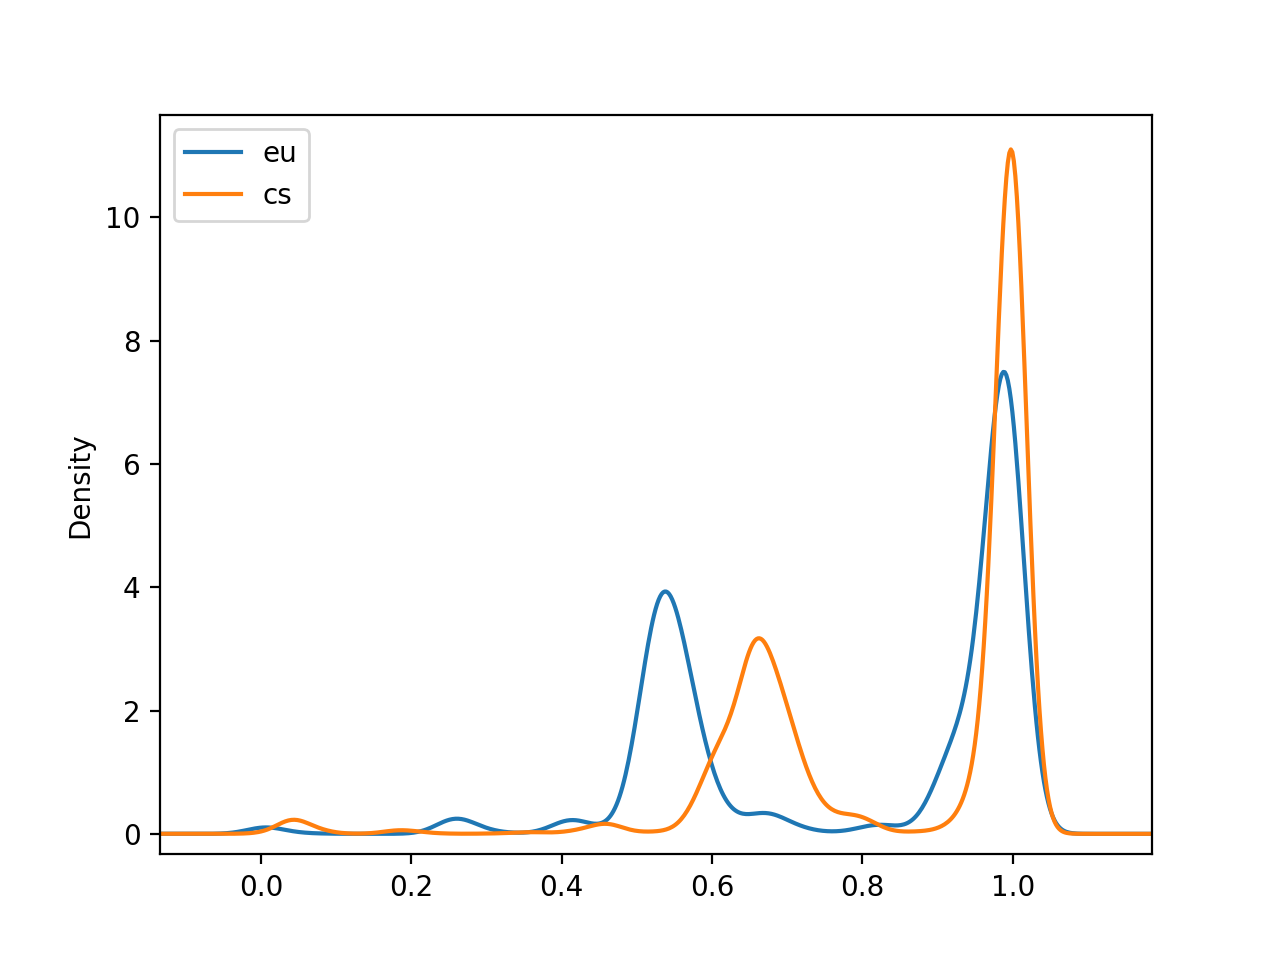
\includegraphics[width=\textwidth]{fig/metric_density.png}
\label{fig:density}
\caption{Gaussian Kernel Density Estimate plot showing the distributions present for each distance metric}
\end{subfigure}
\caption{Showing the evolution from the original overlaid locations, \autoref{fig:morig} to the slightly more accessible (interactively) \autoref{fig:metric}}
\end{figure}


\subsection{Viewing the similarity graph}

One method to simplify this is to convert to the pairwise interaction list into a fully connected graph. Here we have individual species, pulled together by the similarity (geometric mean) between each two nodes.
Unfortunately in being a complete graph of  421 species and 88410 links, this is quite difficult to visualise without forming a \emph{hairball} [fig a]. As a means of filtering the results we trim the weakest links in sequence. This produces rings of densely connected species based on lifetime thresholds which corresponds to the different types of chemsitry species undergo \\



\textbf{Need to find out what the abbreviated names in cri stand for!}. The sizes and species within each ring show similararities to the distance metric plot as would be expected. This provides an alternative representation where graph community detection algorithms such as MCL [ref] can be used to isolate chemistry with different levels of lifetime relationships between them. Unfortunately, as we are interested species with near identical lifetimes, this does not hold a great deal of merit in locating these. 


\begin{figure}[H]

\begin{subfigure}{.33\textwidth}
  \centering
  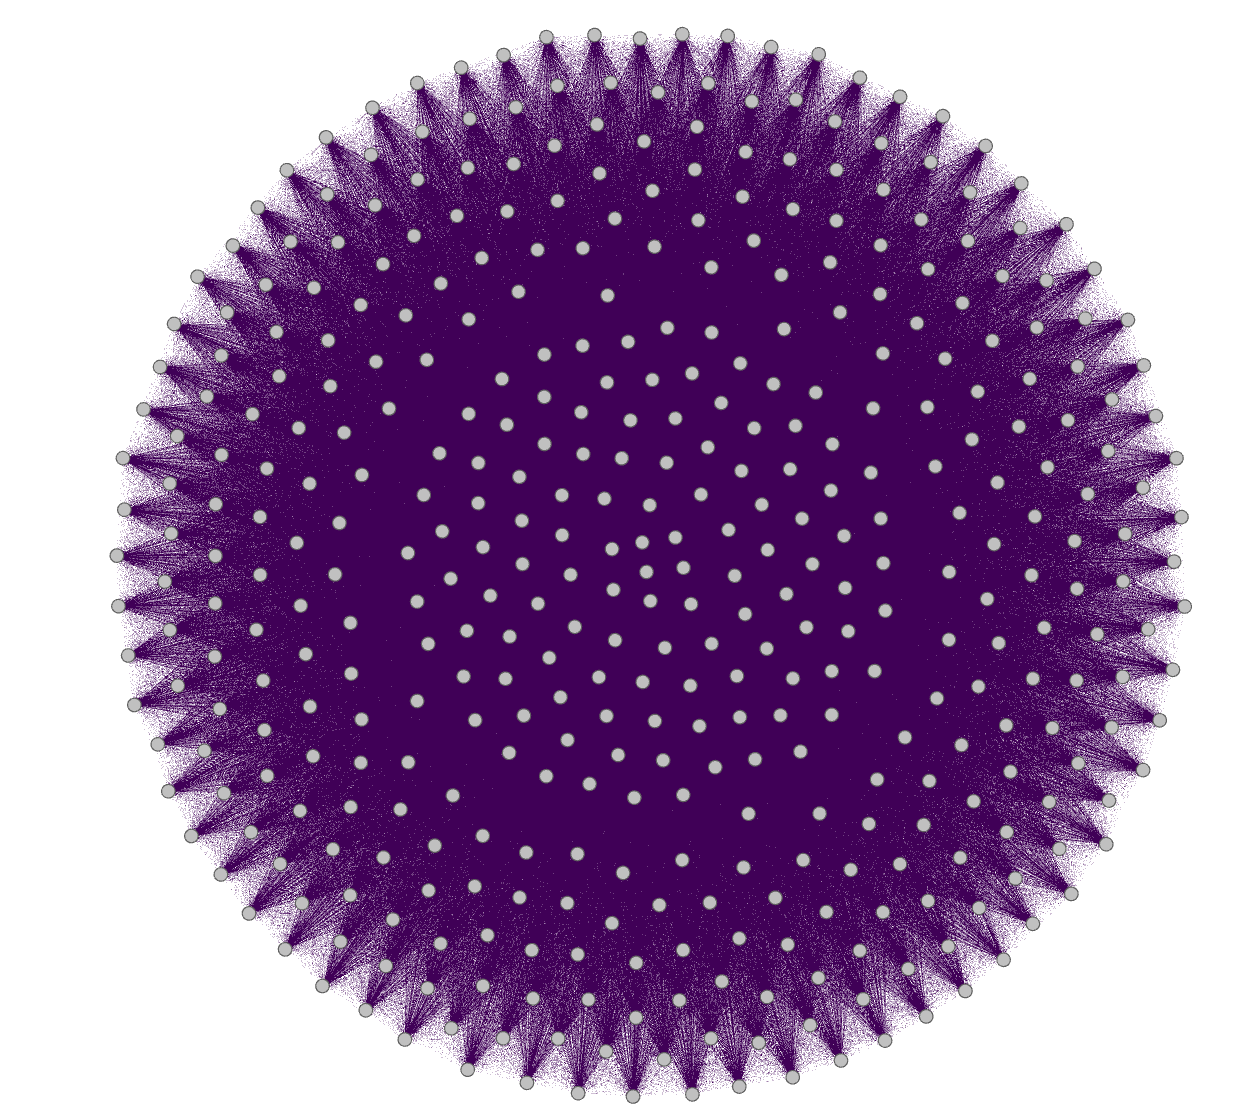
\includegraphics[width=\textwidth]{fig/step1.png}
  \label{fig:orig}
  \caption{Initial connected graph}
\end{subfigure}%
\begin{subfigure}{.33\textwidth}
  \centering
  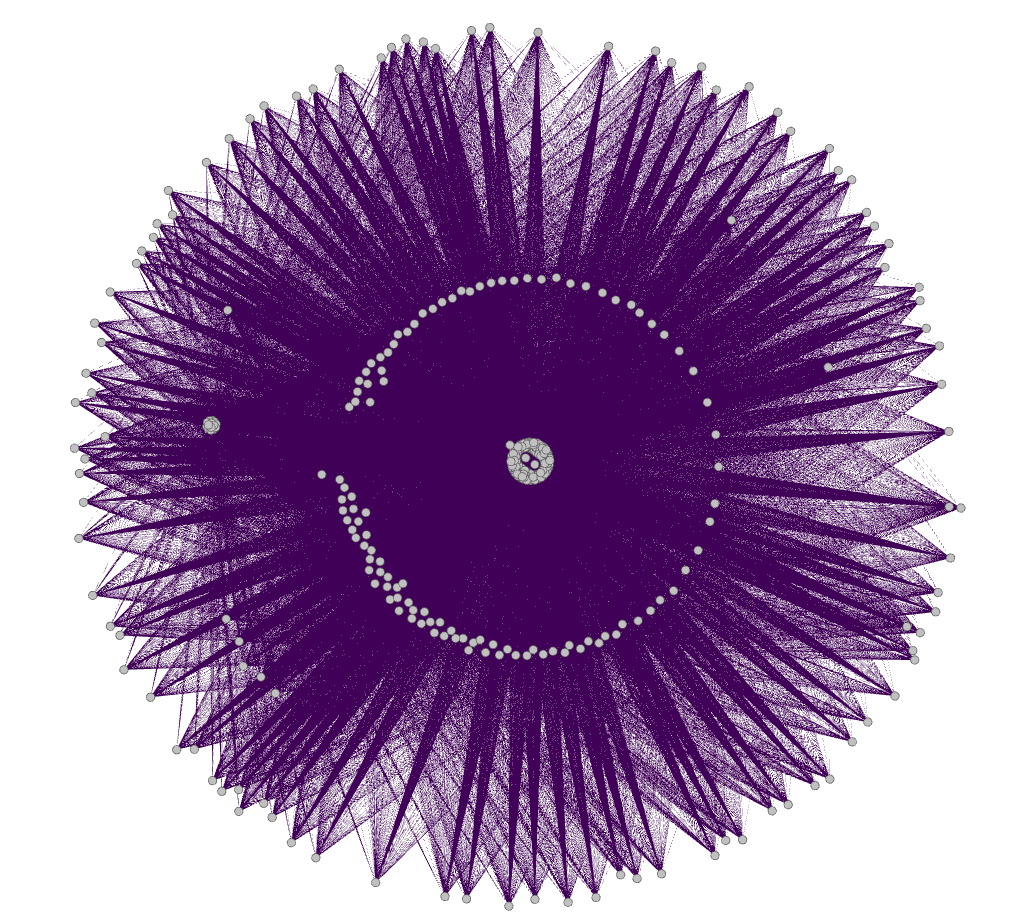
\includegraphics[width=\textwidth]{fig/step2.png}
  \label{fig:pca}
  \caption{Initial graph with trimming ~ half the edges}
\end{subfigure}%
\begin{subfigure}{.33\textwidth}
  \centering
  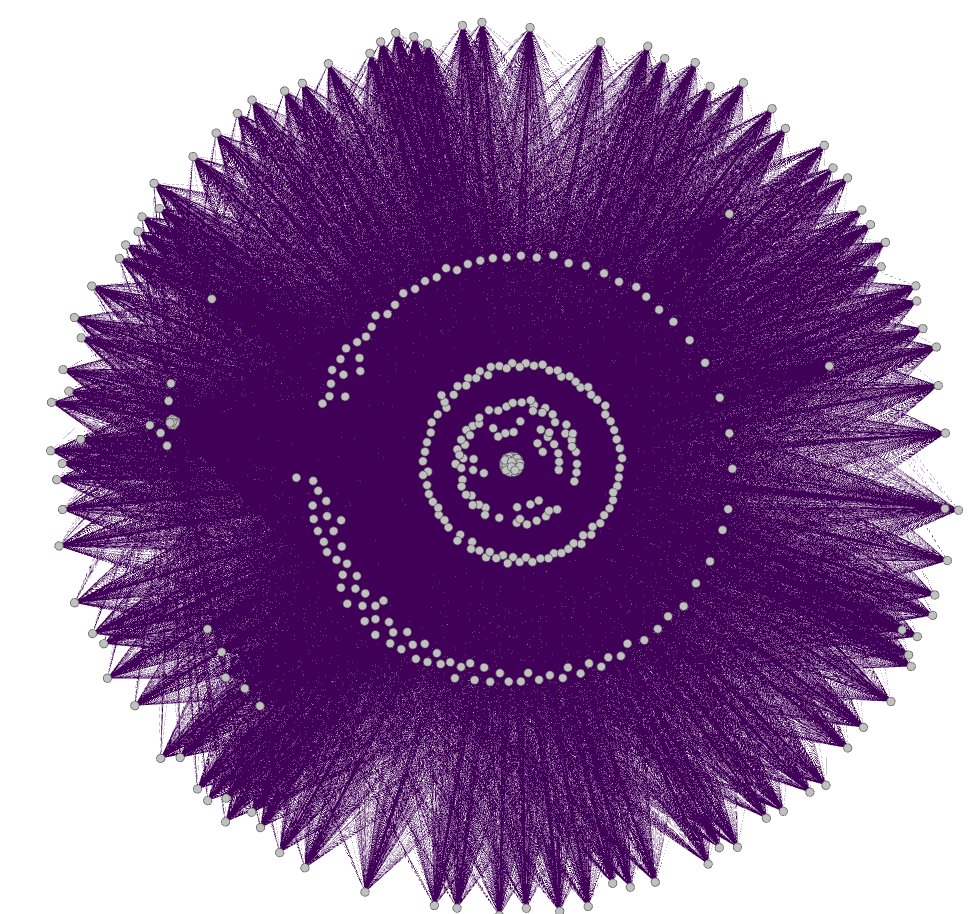
\includegraphics[width=\textwidth]{fig/step3.png}
  \label{fig:ae}
  \caption{Heavy trimming.}
\end{subfigure}%


\caption{A froce graph with progressive trimming of weak, poorly related, edges.}
\end{figure}

\subsubsection{Using MCMC to extract groups}

Need to see what Cri names mean to better explain these. 

